\documentclass[12pt,a4paper]{article}
\renewcommand{\baselinestretch}{1.5} % adding spacing
\usepackage[a4paper, left=3.17cm, right=3.17cm, top=2.54cm, bottom=2.54cm]{geometry} % margins
\usepackage[T1]{fontenc}
\usepackage{mathptmx}
\usepackage{amsmath}
\usepackage{amsfonts}
\usepackage{chemformula}
\usepackage{cite}
\usepackage{svg}
\usepackage{authblk}
\usepackage[colorlinks, linkcolor=black, anchorcolor=black, citecolor=black]{hyperref}
\usepackage{graphicx}
\usepackage{pythonhighlight}
\usepackage{multirow}
\setlength{\parskip}{0.5em}
\title{Made By:}
\author[1]{Eyad Salama}
\author[2]{Nour Hesham}
\affil[1]{Computer and Communication Department, Alexandria University}
\affil[2]{Computer and Communication Department, Alexandria University}


\begin{document}
\newcommand{\HRule}{\rule{\linewidth}{0.5mm}}
    {\centering
    \includesvg[width=180pt]{imgs/logo.svg}
    \quad\\[1.5cm]
    \textsl{\Large University of Alexandria}\\[0.5cm] 
    \textsl{\large Computer and Communication Engineering Department}\\[0.5cm] 
    \makeatletter
    \HRule \\[0.4cm]
    { \huge \bfseries Modulation Classification}\\[0.4cm] 
    \HRule \\[1.5cm]
    % {\large An Assignment submitted for the UoS:}\\[0.5cm]
    {\large \emph{CC484 - Pattern Recognition}}\\[0.5cm]
    }\par
    \maketitle

    \newpage

    \tableofcontents
    
    \newpage
    
    \section{Abstract}
    Modulation identification is an essential component of signal interception analysis, which has long been a study focus in radio communication. Interference in signal transmission gets increasingly problematic as the electromagnetic spectrum environment grows more complicated. This work offers a modulation recognition strategy based on multimodal feature fusion to increase modulation identification performance across various channels.\newline
    In the signal preprocessing stage, various time- and frequency-domain properties are extracted as the network input. The residual shrinkage building unit with channel-wise thresholds (RSBU-CW) was used to create deep convolutional neural networks to extract spatial features that interact in pairs with temporal information collected by LSTM to boost feature diversity.
    Finally, the PNN model was modified to cross-fuse the network's extracted features in order to improve feature complementarity. \newline
    The simulation results show that the proposed technique outperforms existing feature fusion systems in terms of recognition performance, and it can also achieve high recognition performance in multipath fading channels.

    \newpage

    \section{Motivation and Background}
    There are numerous important reasons why machine learning has grown so fast in the last ten years. Algorithms have advanced considerably in a variety of ways, including momentum techniques of gradient descent and advances in regularisation and dropout, among others. Computa-tional power and concurrent programming models to fully use it have also increased substantially, thanks in large part to high-level languages that compile quickly to contemporary GPU implementations.\newline
    Another significant enabler has been access to big and well-curated datasets, which has allowed individuals to quickly compare ideas, test new techniques, and train models with enormous parameter spaces.\newline
    Many of the most recent improvements in machine learning are being driven by researchers in computer vision, speech recognition, natural language processing, medical images, and finance. Unfortunately, radio signal processing has been conspicuously absent from most of this recent work;\newline
    yet, the potential for applying recent improvements in machine learning to the radio domain is huge right now. Researchers are increasingly studying these approaches, however there are no clear benchmarks or available datasets for evaluating advancements, as seen in other application fields.
    \newpage
    
    \section{Introduction}
    

    Because of the high demand for wireless data researchers have recently focused on developing smart radios that can coexist. \newline 
    The concept of Cognitive Radios was initially proposed by Mitola. \newline 
    His suggested model has two sorts of users: licenced users or primary users (PUs) who have priority in using the spectrum bands in question, and unlicensed users or secondary users (SUs) who are permitted to broadcast in the specified frequency band as long as no interference occurs on the PUs side. \newline
    A CR's capacity to scan the spectrum to determine the type of users in the system is one of the listed features. \newline
    Following that, it will adjust its broadcast to avoid interference with neighbouring users. \newline
    To correctly categorise these users, the CR must begin a learning phase in which he studies the transmission properties of every incoming signal. The modulation technique utilised is one of the most important aspects of any signal. \newline
    To properly recover the signal, the transmitter and receiver must agree on the modulation scheme as part of the physical layer of any wireless radio. \newline
    A number of neural network types were also employed. Among the most plausible methods were Long Term Short Memory and Residual Networks (ResNet). \newline
    Another approach employed in was making a vanilla RNN instead of using the LSTM but the first approach had better results. \newline
    We also tried implementing an CNN neural network and most of the times it performed better than the vanilla RNN neural network\newline
    TODO:\newline
    The last approach that we tried was using a CONV-LSTM neural network \newline

    \newpage

    \section{Modulations and Neural Networks}
    As we discussed in the previous section we used Three approaches but before discussing each architecture we need an brief introduction about our DataSet that we used.
    \subsection{About Our DataSet}
    A synthetic dataset of 10 modulations created with GNU Radio.
    This is a variable-SNR dataset with modest LO drift, light fading, and a variety of labelled SNR increments for assessing performance in various signal and noise power circumstances. \newline
    We have 20 SNR values [-18, -16,... 18] and 10 modulation types (8 digital and 2 analog modulation types). \newline
    So in total we have 200 combinations and each combination has 6000 samples so, in total we have 1.2M samples as our dataset. In this experiment we only care about the modulation type and not the corresponding SNR value so our neural networks is going to have 10 heads (each head for a specific modulation type)

    \newpage
    
    \subsection{OurCNN}
         \begin{center}
         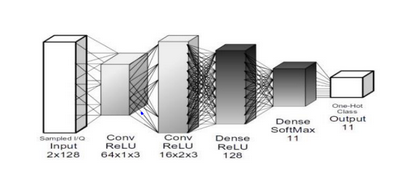
\includegraphics{imgs/cnn.png}
        \end{center}
        \begin{python}
class OurCNN(nn.Module):
    def __init__(self, num_classes, input_shape=(2, 128)):
        super().__init__()
        self.num_classes = num_classes
        self.input_shape = input_shape
        self.batchnorm = nn.BatchNorm2d(2)
        self.conv1 = nn.Sequential(
            nn.Conv2d(
                in_channels=1,
                out_channels=64,
                kernel_size=(1, 3),
                stride=1,
                padding='same'
            ),
            nn.BatchNorm2d(64),
            nn.ReLU(),
        )
        self.conv2 = nn.Sequential(
            nn.Conv2d(
                in_channels=64,
                out_channels=16,
                kernel_size=(2, 3),
                stride=1,
                padding='same'
            ),
            nn.BatchNorm2d(16),
            nn.ReLU()
        )
        self.relu = nn.ReLU()
        self.flatten = nn.Flatten()
        self.softmax = nn.Softmax(dim=1)
        self.dropout = nn.Dropout(p=0.5)
        n_size = self._get_conv_output(self.input_shape)
        self.linear_1 = nn.Linear(n_size, 128)
        self.linear_2 = nn.Linear(128, 10)

    def forward(self, input):
        x = torch.unsqueeze(input, dim=1)
        x = self.conv1(x)
        x = self.dropout(x)
        x = self.conv2(x)
        x = self.dropout(x)
        x = self.flatten(x)
        x = self.linear_1(x)
        x = self.relu(x)
        x = self.linear_2(x)
        #x = self.softmax(x)
        return x

    def _get_conv_output(self, shape):
        bs = 1
        input_data = Variable(torch.rand(bs, *shape))
        input_data = torch.unsqueeze(input_data, dim=1)
        x = self.conv1(input_data)
        x = self.conv2(x)
        x = self.flatten(x)
        n_size = x.data.view(bs, -1).size(1)
        return n_size
\end{python}
    \newpage
    

    \subsection{OurRNN}
      \begin{center}
            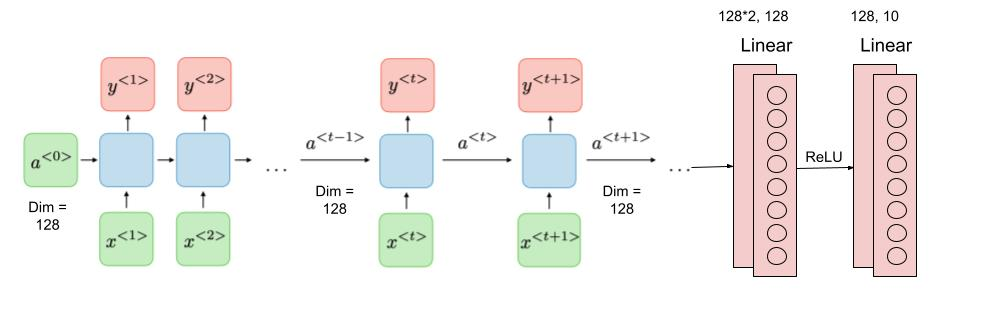
\includegraphics[width= 400pt]{imgs/rnn.jpg}
        \end{center}
    \begin{python}
    class OurRNN(nn.Module):

    def __init__(self, num_classes, input_dim, hidden_dim):
        super().__init__()
        self.device = torch.device("cuda:0"if torch.cuda.is_available()else"cpu")
        self.num_classes = num_classes
        self.input_dim = input_dim
        self.hidden_dim = hidden_dim
        self.batchnorm = nn.BatchNorm1d(2)
        self.rnn = nn.RNN(
            input_size=input_dim, 
            hidden_size=hidden_dim,
            num_layers = 1, 
            batch_first=True,
            nonlinearity='tanh')
        self.fc1 = nn.Linear(hidden_dim*2, 128)
        self.fc2 = nn.Linear(128, num_classes)
        self.relu = nn.ReLU()
    def forward(self, x):
        x = self.batchnorm(x)
        h0 = Variable(torch.zeros(1, x.size(0), self.hidden_dim)).to(self.device)
        out, hn = self.rnn(x, h0)
        out = out.contiguous().view(x.size(0),-1)
        out = self.fc1(out)
        out = self.relu(out)
        out = self.fc2(out)
        return out
    \end{python}
    \newpage

    \subsection{OurLSTM}

    \begin{center}
            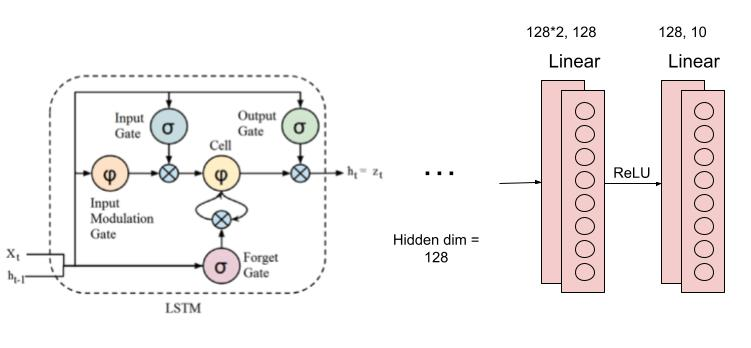
\includegraphics[width= 400pt]{imgs/lstm.jpg}
        \end{center}
    
    \begin{python}
    class OurLSTM(nn.Module):

    def __init__(self, num_classes, input_dim, hidden_dim):
        super().__init__()
        self.device = torch.device("cuda:0" if torch.cuda.is_available() else "cpu")
        self.num_classes = num_classes
        self.input_dim = input_dim
        self.hidden_dim = hidden_dim
        self.batchnorm = nn.BatchNorm1d(2)
        self.lstm = nn.LSTM(
            input_size=input_dim, 
            hidden_size=hidden_dim,
            num_layers = 1, 
            batch_first=True)
        self.fc1 = nn.Linear(hidden_dim*2, 128)
        self.fc2 = nn.Linear(128, num_classes)
        self.relu = nn.ReLU()

    def forward(self, x):
        x = self.batchnorm(x)
        h0 = Variable(torch.zeros(1, x.size(0), self.hidden_dim)).to(self.device)
        c0 = Variable(torch.zeros(1, x.size(0), self.hidden_dim)).to(self.device)
        out, (hn, cn) = self.lstm(x, (h0,c0))
        out = out.contiguous().view(x.size(0),-1)
        out = self.fc1(out)
        out = self.relu(out)
        out = self.fc2(out)
        return out
    \end{python}
    \newpage

    \subsection{RNN vs LSTM}
        \begin{center}
            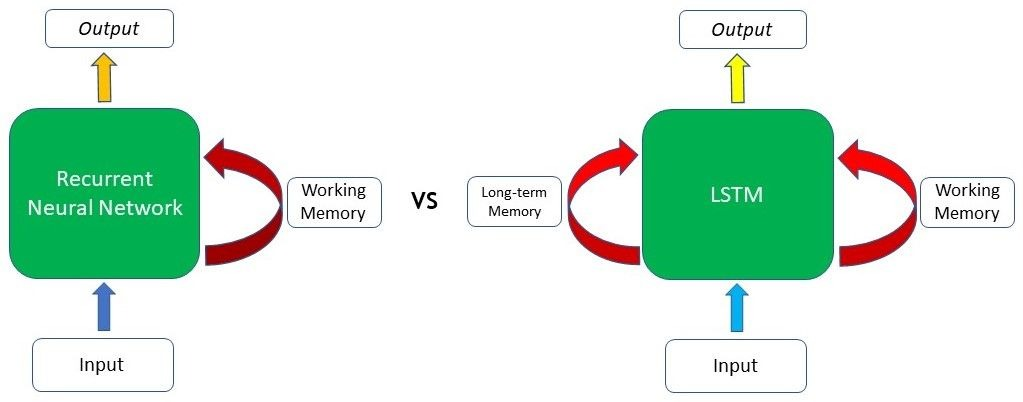
\includegraphics[width= 400pt]{imgs/rnnlstm.jpg}
        \end{center}

        \subsection{RNNs have recurrent connections and/or layers}
        Depending on the context, you may define a recurrent neural network (RNN) or a long short-term memory (LSTM) at different degrees of abstraction. An RNN, for example, might be defined as any neural network with one or more recurrent (or cyclic) connections. Layer l of neural network N is a recurrent layer since it includes units (or neurons) with recurrent connections, whereas N is not.\newline
        may not only have recurring layers (for example, it may also be composed of feedforward layers, i.e. layers with units that contain only feedforward connections).\newline
        In any event, a recurrent neural network (RNN) is generally always referred to as a neural network (NN) rather than a layer (this should also be obvious from the name).
        \newpage
        \subsection{LSTM can refer to a unit, layer or neural network}
        However, depending on the context, the word "LSTM" might refer to an LSTM unit (or neuron), an LSTM layer (a collection of LSTM units), or an LSTM neural network (a neural network with LSTM units or layers).\newline
        LSTMs are another name for neural networks incorporating LSTM units (plural version of LSTM).
        \begin{center}
         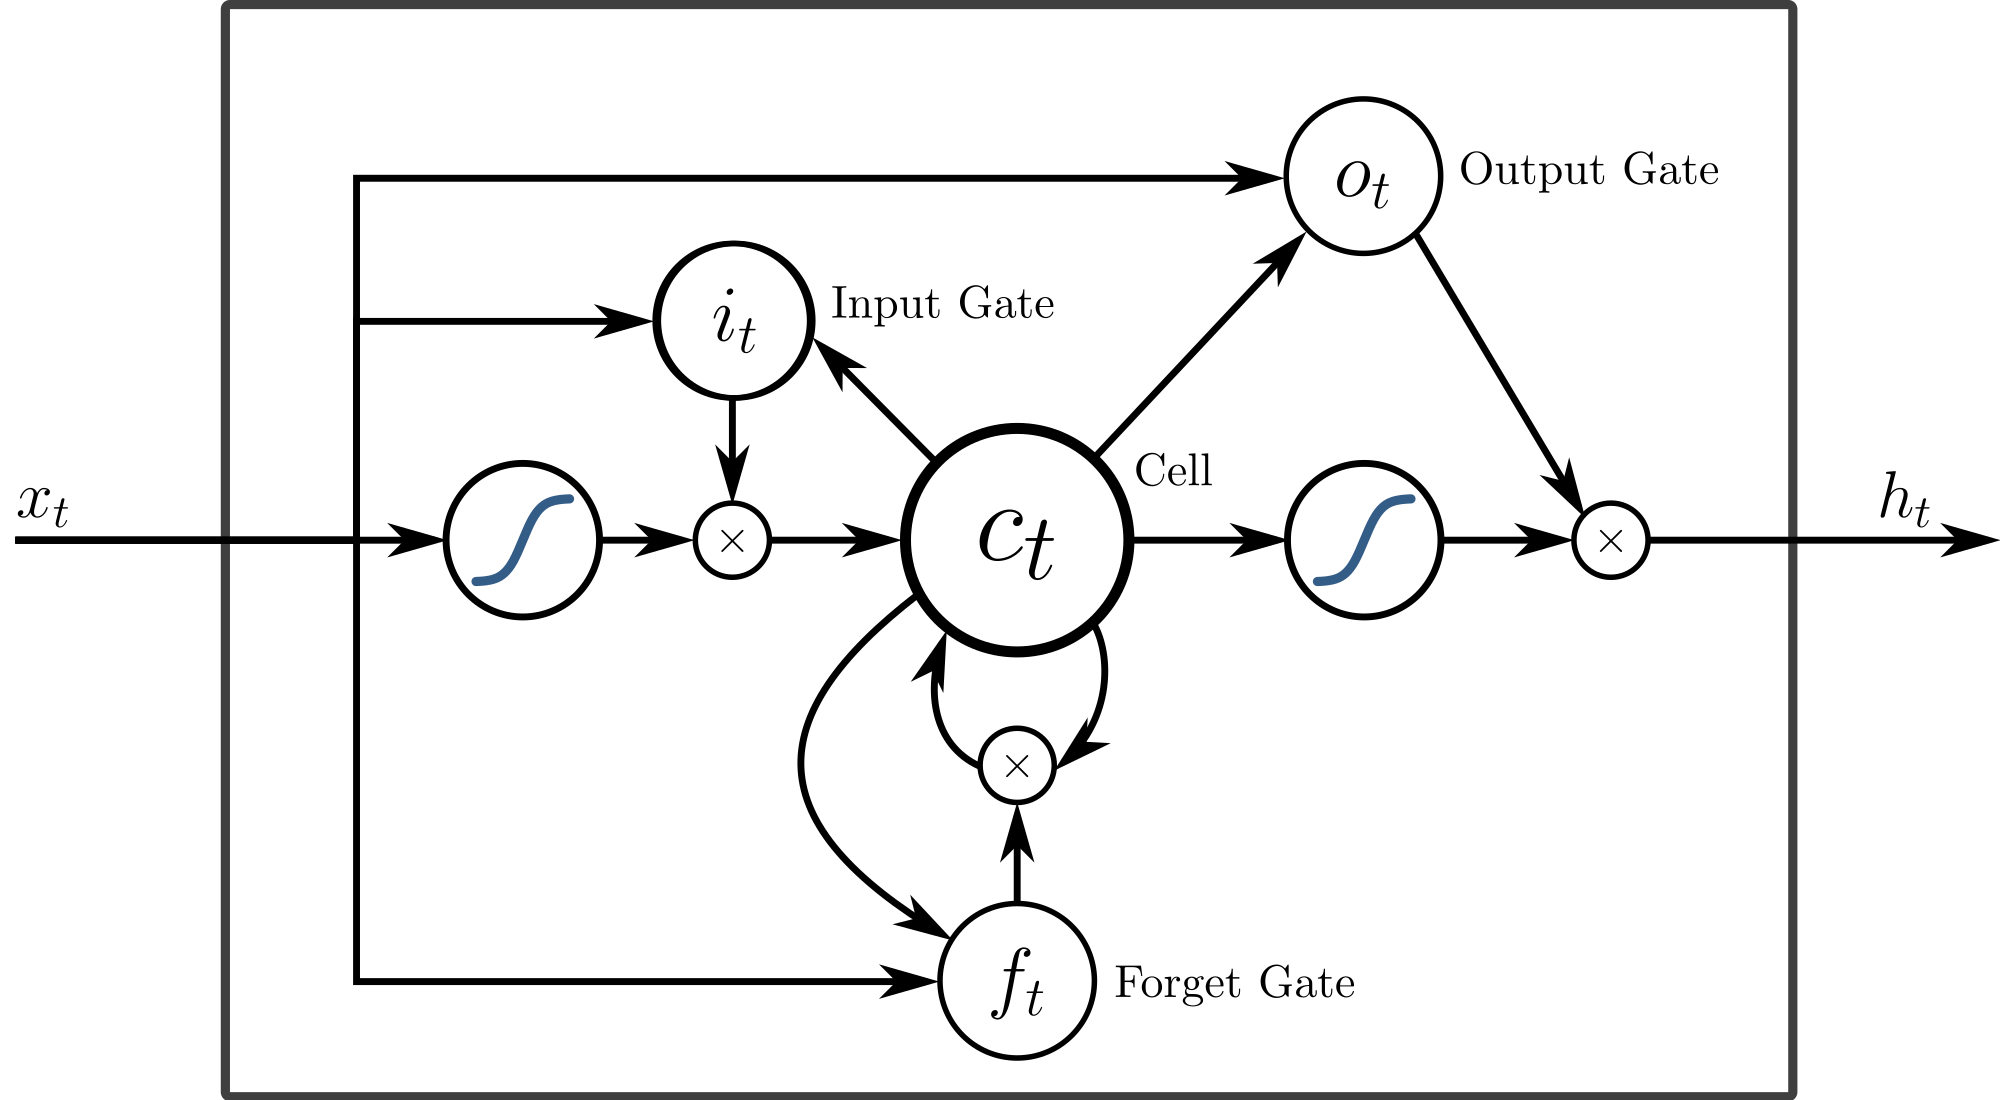
\includegraphics[width=320pt]{imgs/lstm.png}
        \end{center}
        we can see from this diagram that an LSTM unit (or layer) is composed of gates \newline
        1. i -> input gate. \newline
        2. o -> output gate. \newline
        3. f -> forget gate
    \subsection{When should you use RNNs and LSTMs?}
    RNNs are particularly well-suited for jobs involving sequences (thanks to the recurrent connections). They are frequently employed in machine translation, for example, when the sequences represent phrases or words. \newline
    In practise, an LSTM is frequently used instead of a vanilla (or standard) RNN since it is more computationally efficient. \newline
    In reality, the LSTM was developed to address a difficulty that regular RNNs face, namely the vanishing gradient problem.
    \newpage

    \section{Results and Discussion}
    \subsection{Train all models on different feature spaces, no hyperparameter tweaking, find best combination, and tweak hyperparameters on diff models}
    \begin{table}[!ht]
    \raggedright
    \begin{tabular}{|l|l|l|l|l|l|}
    \hline
        \textbf{Arch} & CNN & RNN, hid = 128 & LSTM, hid = 128 & CNN & RNN \\ \hline
        \textbf{LR} & 1.00E-03 & 1.00E-03 & 1.00E-03 & 1.00E-03 & 1.00E-03 \\ \hline
        \textbf{Batch} & 256 & 256 & 256 & 256 & 256 \\ \hline
        \textbf{Epochs} & 10 & 10 & 10 & 10 & 10 \\ \hline
        \textbf{Features} & Raw & Raw & Raw & Derivative & Derivative \\ \hline
        \textbf{Acc (train, val) E} & 0.545, 0.512 & 0.487, 0.481 & 0.537, 0.5159 & 0.3705, 0.354 & 0.317, 0.195 \\ \hline
        \textbf{F1 (train, val) E} & 0.548, 0.518 & 0.499, 0.495 & 0.55, 0.54 & 0.3953, 0.401 & 0.3327, 0.2438 \\ \hline
        \textbf{Acc (train, val) S} & 0.652, 0.625 & 0.585, 0.57 & 0.666, 0.6875 & 0.503, 0.5 & 0.414, 0.375 \\ \hline
        \textbf{F1 (train, val) S} & 0.658, 0.642 & 0.587, 0.658 & 0.6837, 0.684 & 0.559, 0.494 & 0.476, 0.405 \\ \hline
    \end{tabular}
\end{table}

    \begin{table}[!ht]
    \raggedright
    \begin{tabular}{|l|l|}
    \hline
        \textbf{Arch} & LSTM \\ \hline
        \textbf{LR} & 1.00E-03 \\ \hline
        \textbf{Batch} & 256 \\ \hline
        \textbf{Epochs} & 10 \\ \hline
        \textbf{Features} & Derivative \\ \hline
        \textbf{Acc (train, val) E} & 0.334, 0.328 \\ \hline
        \textbf{F1 (train, val) E} & 0.3605, 0.35 \\ \hline
        \textbf{Acc (train, val) S} & 0.4414, 0.4257 \\ \hline
        \textbf{F1 (train, val) S} & 0.4698, 0.443 \\ \hline
    \end{tabular}
    \end{table}
    \newpage
    \subsection{Train best feature space "raw" with diff learning rates on diff models}
    \begin{table}[!ht]
    \raggedright
    \begin{tabular}{|l|l|l|l|l|l|}
    \hline
        \textbf{Arch} & CNN & RNN & LSTM & CNN & RNN \\ \hline
        \textbf{LR} & 1.00E-04 & 1.00E-04 & 1.00E-04 & 5.00E-04 & 5.00E-04 \\ \hline
        \textbf{Batch} & 256 & 256 & 256 & 256 & 256 \\ \hline
        \textbf{Epochs} & 10 & 10 & 10 & 10 & 10 \\ \hline
        \textbf{Features} & Raw & Raw & Raw & Raw & Raw \\ \hline
        \textbf{Acc (train, val) E} & 0.51, 0.5527 & 0.371, 0.373 & 0.415, 0.415 & 0.514, 0.545 & 0.395, 0.3902 \\ \hline
        \textbf{F1 (train, val) E} & 0.4738, 0.5244 & 0.313, 0.329 & 0.349, 0.366 & 0.4907, 0.511 & 0.3506, 0.416 \\ \hline
        \textbf{Acc (train, val) S} & 0.617, 0.75 & 0.4609, 0.625 & 0.5833, 0.625 & 0.644, 0.8125 & 0.496, 0.75 \\ \hline
        \textbf{F1 (train, val) S} & 0.626, 0.7455 & 0.492, 0.659 & 0.5816, 0.6406  & 0.647, 0.7927 & 0.5416, 0.7946 \\ \hline
    \end{tabular}
\end{table}
\begin{table}[!ht]
    \raggedright
    \begin{tabular}{|l|l|l|l|l|}
    \hline
        \textbf{Arch} & LSTM & CNN & RNN & LSTM \\ \hline
        \textbf{LR} & 5.00E-04 & 5.00E-03 & 5.00E-03 & 5.00E-03 \\ \hline
        \textbf{Batch} & 256 & 256 & 256 & 256 \\ \hline
        \textbf{Epochs} & 10 & 10 & 10 & 10 \\ \hline
        \textbf{Features} & Raw & Raw & Raw & Raw \\ \hline
        \textbf{Acc (train, val) E} & 0.49, 0.479 & 0.474, 0.38 & 0.403, 0.414 & 0.498, 0.518 \\ \hline
        \textbf{F1 (train, val) E} & 0.427, 0.435 & 0.459, 0.269 & 0.3688, 0.386 & 0.458, 0.481 \\ \hline
        \textbf{Acc (train, val) S} & 0.597, 0.6875 & 0.574, 0.6875 & 0.519, 0.625 & 0.605, 0.8125 \\ \hline
        \textbf{F1 (train, val) S} & 0.6222, 0.709 & 0.588, 0.78125 & 0.557, 0.717 & 0.616, 0.803 \\ \hline
    \end{tabular}
\end{table}
    \newpage
    \subsection{Testing best models on each SNR alone}
    \subsubsection{MODEL: OurCNN LR=1e-04}
    \begin{table}[!ht]
    \raggedright
    \begin{tabular}{|l|l|}
    \hline
        SNR & Accuracy \\ \hline
        -20 & 0.1171875 \\ \hline
        -18 & 0.1328125 \\ \hline
        -16 & 0.140625 \\ \hline
        -14 & 0.1875 \\ \hline
        -12 & 0.2109375 \\ \hline
        -10 & 0.29296875 \\ \hline
        -8 & 0.375 \\ \hline
        -6 & 0.51171875 \\ \hline
        -4 & 0.609375 \\ \hline
        -2 & 0.7421875 \\ \hline
        0 & 0.7734375 \\ \hline
        2 & 0.75 \\ \hline
        4 & 0.78515625 \\ \hline
        6 & 0.8203125 \\ \hline
        8 & 0.80859375 \\ \hline
        10 & 0.80078125 \\ \hline
        12 & 0.7734375 \\ \hline
        14 & 0.82421875 \\ \hline
        16 & 0.81640625 \\ \hline
        18 & 0.76171875 \\ \hline
    \end{tabular}
\end{table}
    \newpage
    \subsubsection{MODEL: OurCNN LR=1e-04}
    \begin{table}[!ht]
    \raggedright
    \begin{tabular}{|l|l|}
    \hline
        SNR & Accuracy \\ \hline
        -20 & 0.109375 \\ \hline
        -18 & 0.11328125 \\ \hline
        -16 & 0.109375 \\ \hline
        -14 & 0.1328125 \\ \hline
        -12 & 0.16015625 \\ \hline
        -10 & 0.20703125 \\ \hline
        -8 & 0.27734375 \\ \hline
        -6 & 0.42578125 \\ \hline
        -4 & 0.54296875 \\ \hline
        -2 & 0.703125 \\ \hline
        0 & 0.66015625 \\ \hline
        2 & 0.73046875 \\ \hline
        4 & 0.7578125 \\ \hline
        6 & 0.78125 \\ \hline
        8 & 0.765625 \\ \hline
        10 & 0.80859375 \\ \hline
        12 & 0.72265625 \\ \hline
        14 & 0.75 \\ \hline
        16 & 0.7734375 \\ \hline
        18 & 0.75390625 \\ \hline
    \end{tabular}
\end{table}
    \newpage
    \subsubsection{MODEL: OurRNN LR=1e-03}
    \begin{table}[!ht]
    \raggedright
    \begin{tabular}{|l|l|}
    \hline
        SNR & Accuracy \\ \hline
        -20 & 0.09375 \\ \hline
        -18 & 0.10546875 \\ \hline
        -16 & 0.1171875 \\ \hline
        -14 & 0.16015625 \\ \hline
        -12 & 0.1953125 \\ \hline
        -10 & 0.33203125 \\ \hline
        -8 & 0.40625 \\ \hline
        -6 & 0.4296875 \\ \hline
        -4 & 0.609375 \\ \hline
        -2 & 0.71484375 \\ \hline
        0 & 0.76953125 \\ \hline
        2 & 0.73828125 \\ \hline
        4 & 0.77734375 \\ \hline
        6 & 0.8125 \\ \hline
        8 & 0.79296875 \\ \hline
        10 & 0.81640625 \\ \hline
        12 & 0.78515625 \\ \hline
        14 & 0.80078125 \\ \hline
        16 & 0.8125 \\ \hline
        18 & 0.76953125 \\ \hline
    \end{tabular}
\end{table}
\newpage

    \subsubsection{MODEL: OurRNN_LR=5e-044}
    \begin{table}[!ht]
    \raggedright
    \begin{tabular}{|l|l|}
    \hline
        SNR & Accuracy \\ \hline
        -20 & 0.14453125 \\ \hline
        -18 & 0.1484375 \\ \hline
        -16 & 0.1328125 \\ \hline
        -14 & 0.16796875 \\ \hline
        -12 & 0.203125 \\ \hline
        -10 & 0.23828125 \\ \hline
        -8 & 0.390625 \\ \hline
        -6 & 0.41015625 \\ \hline
        -4 & 0.49609375 \\ \hline
        -2 & 0.50390625 \\ \hline
        0 & 0.61328125 \\ \hline
        2 & 0.44140625 \\ \hline
        4 & 0.5546875 \\ \hline
        6 & 0.5546875 \\ \hline
        8 & 0.55078125 \\ \hline
        10 & 0.515625 \\ \hline
        12 & 0.50390625 \\ \hline
        14 & 0.5546875 \\ \hline
        16 & 0.5234375 \\ \hline
        18 & 0.49609375 \\ \hline
    \end{tabular}
\end{table}
    \newpage
    \subsubsection{MODEL: OurLSTM_LR=1e-03}
    \begin{table}[!ht]
    \raggedright
    \begin{tabular}{|l|l|}
    \hline
        SNR & Accuracy \\ \hline
        -20 & 0.10546875 \\ \hline
        -18 & 0.1328125 \\ \hline
        -16 & 0.1640625 \\ \hline
        -14 & 0.1875 \\ \hline
        -12 & 0.2265625 \\ \hline
        -10 & 0.34765625 \\ \hline
        -8 & 0.39453125 \\ \hline
        -6 & 0.5 \\ \hline
        -4 & 0.60546875 \\ \hline
        -2 & 0.6484375 \\ \hline
        0 & 0.76953125 \\ \hline
        2 & 0.66796875 \\ \hline
        4 & 0.734375 \\ \hline
        6 & 0.77734375 \\ \hline
        8 & 0.76171875 \\ \hline
        10 & 0.734375 \\ \hline
        12 & 0.69140625 \\ \hline
        14 & 0.75 \\ \hline
        16 & 0.70703125 \\ \hline
        18 & 0.6796875 \\ \hline
    \end{tabular}
\end{table}
    \newpage
    \subsubsection{MODEL: |MODEL: OurLSTM_LR=5e-04}
    \begin{table}[!ht]
    \raggedright
    \begin{tabular}{|l|l|}
    \hline
        SNR & Accuracy \\ \hline
        -20 & 0.15625 \\ \hline
        -18 & 0.14453125 \\ \hline
        -16 & 0.14453125 \\ \hline
        -14 & 0.140625 \\ \hline
        -12 & 0.203125 \\ \hline
        -10 & 0.3203125 \\ \hline
        -8 & 0.421875 \\ \hline
        -6 & 0.48046875 \\ \hline
        -4 & 0.55078125 \\ \hline
        -2 & 0.63671875 \\ \hline
        0 & 0.703125 \\ \hline
        2 & 0.64453125 \\ \hline
        4 & 0.69140625 \\ \hline
        6 & 0.75 \\ \hline
        8 & 0.73828125 \\ \hline
        10 & 0.6875 \\ \hline
        12 & 0.67578125 \\ \hline
        14 & 0.69140625 \\ \hline
        16 & 0.68359375 \\ \hline
        18 & 0.66015625 \\ \hline
    \end{tabular}
\end{table}
    \newpage
    
    \subsection{Using Raw time series}
    \begin{center}
         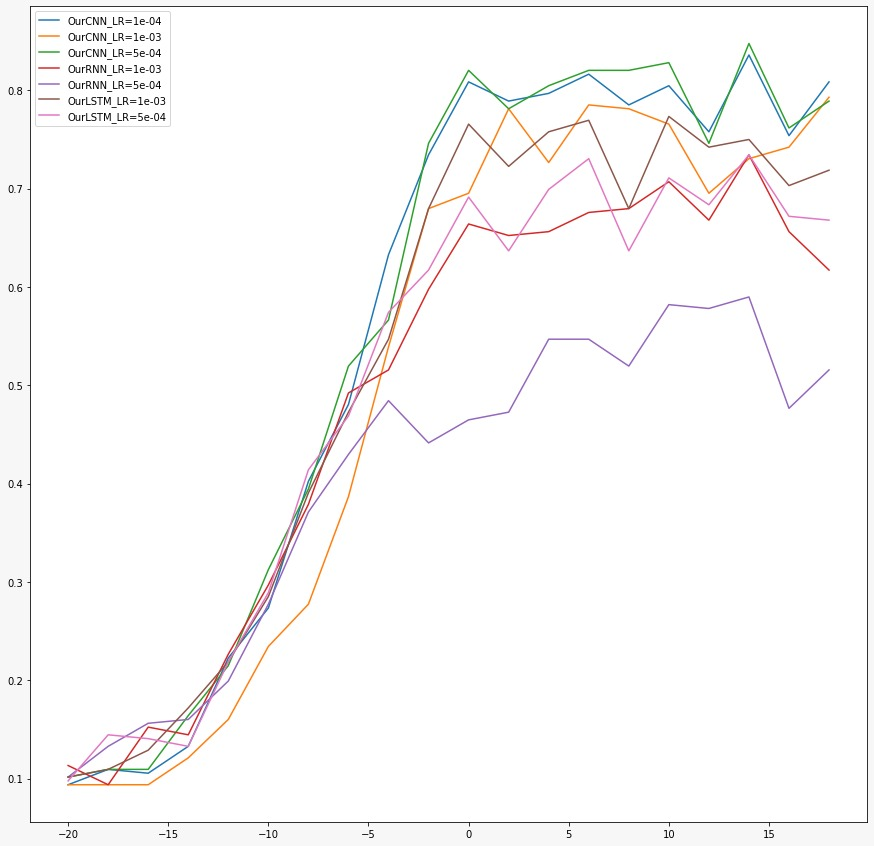
\includegraphics[width=320pt]{imgs/graph1.jpg}
        \end{center}
        \subsection{Using First Derivative in time}
    \begin{center}
         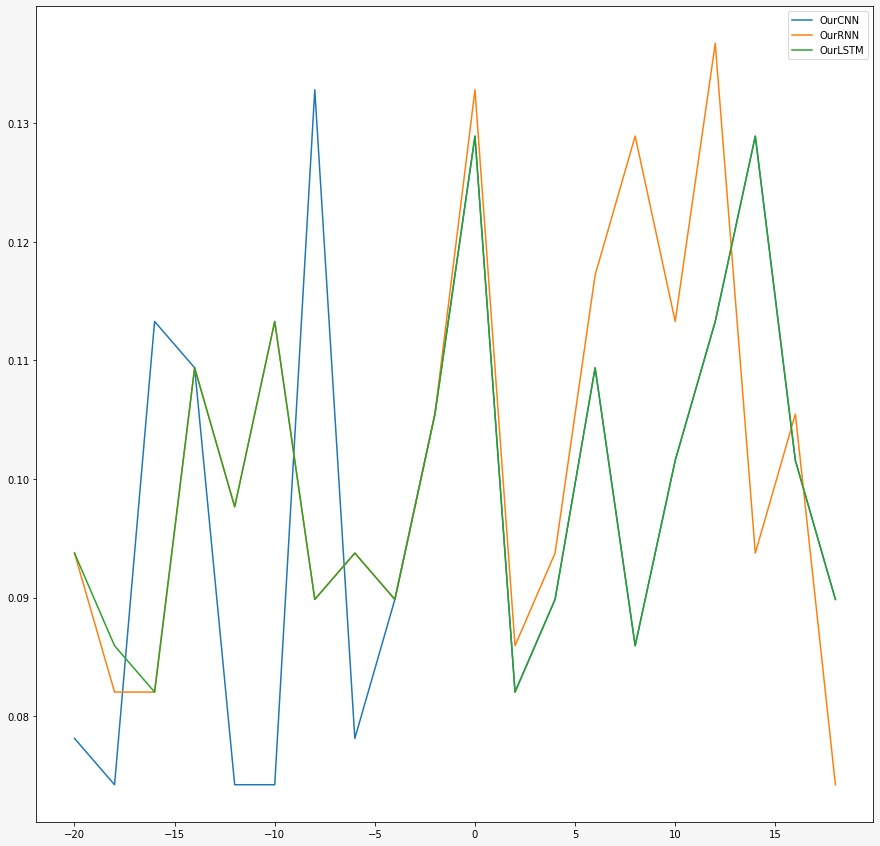
\includegraphics[width=320pt]{imgs/dt.jpg}
        \end{center}
        \newpage
        \subsection{Confusion Matrices}
        
\subsubsection{At SNR -20}
\begin{center}
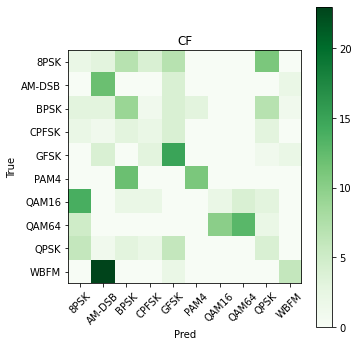
\includegraphics[width=320pt]{imgs/snrs/snr6.png}
\end{center}

\subsubsection{At SNR -18}
\begin{center}
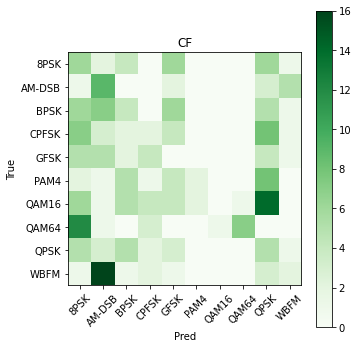
\includegraphics[width=320pt]{imgs/snrs/snr4.png}
\end{center}

\subsubsection{At SNR -16}
\begin{center}
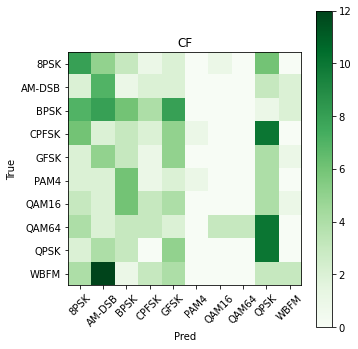
\includegraphics[width=320pt]{imgs/snrs/snr3.png}
\end{center}

\subsubsection{At SNR -14}
\begin{center}
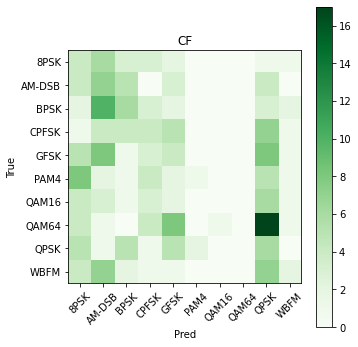
\includegraphics[width=320pt]{imgs/snrs/snr2.png}
\end{center}

\subsubsection{At SNR -12}
\begin{center}
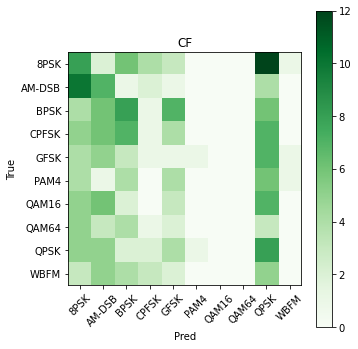
\includegraphics[width=320pt]{imgs/snrs/snr1.png}
\end{center}

\subsubsection{At SNR -10}
\begin{center}
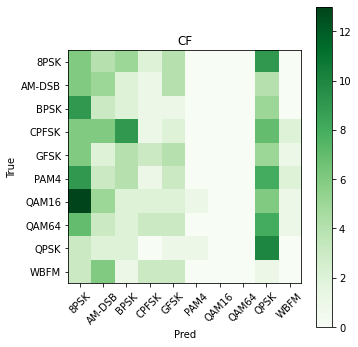
\includegraphics[width=320pt]{imgs/snrs/snr0.png}
\end{center}

\subsubsection{At SNR -8}
\begin{center}
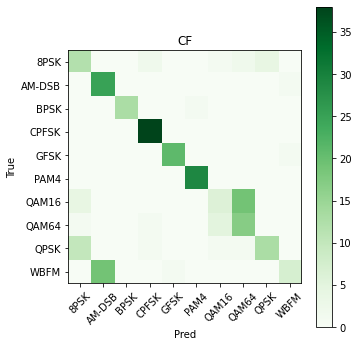
\includegraphics[width=320pt]{imgs/snrs/snr9.png}
\end{center}
\subsubsection{At SNR -6}
\begin{center}
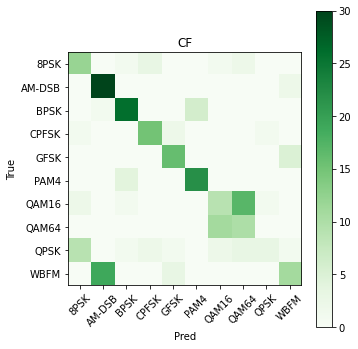
\includegraphics[width=320pt]{imgs/snrs/snr8.png}
\end{center}
\subsubsection{At SNR -4}
\begin{center}
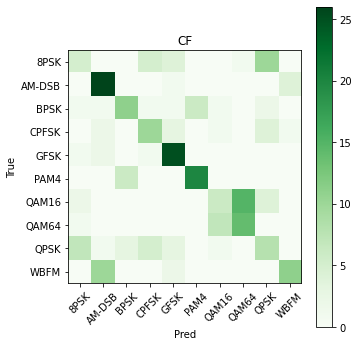
\includegraphics[width=320pt]{imgs/snrs/snr7.png}
\end{center}
\subsubsection{At SNR -2}
\begin{center}
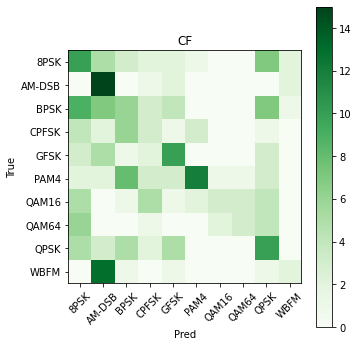
\includegraphics[width=320pt]{imgs/snrs/snr5.png}
\end{center}
\subsubsection{At SNR 0}
\begin{center}
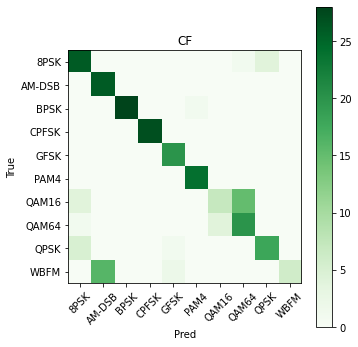
\includegraphics[width=320pt]{imgs/snrs/snr10.png}
\end{center}
\subsubsection{At SNR 2}
\begin{center}
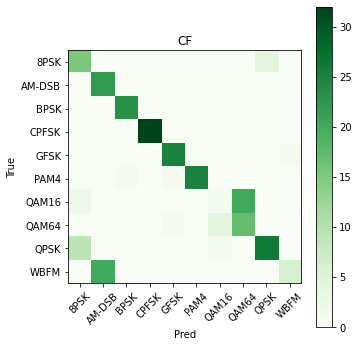
\includegraphics[width=320pt]{imgs/snrs/snr16.png}
\end{center}
\subsubsection{At SNR 4}
\begin{center}
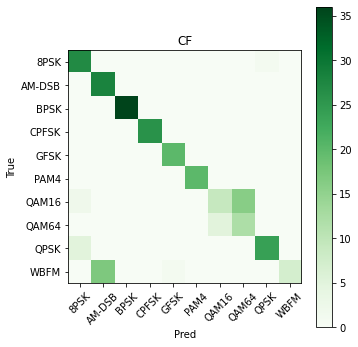
\includegraphics[width=320pt]{imgs/snrs/snr17.png}
\end{center}
\subsubsection{At SNR 6}
\begin{center}
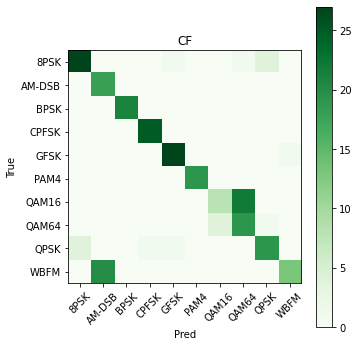
\includegraphics[width=320pt]{imgs/snrs/snr18.png}
\end{center}
\subsubsection{At SNR 8}
\begin{center}
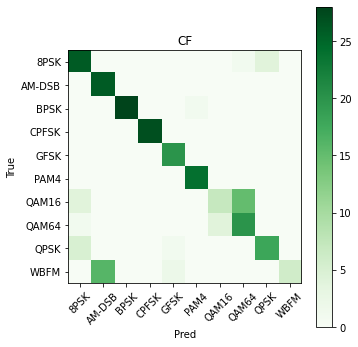
\includegraphics[width=320pt]{imgs/snrs/snr10.png}
\end{center}
\subsubsection{At SNR 10}
\begin{center}
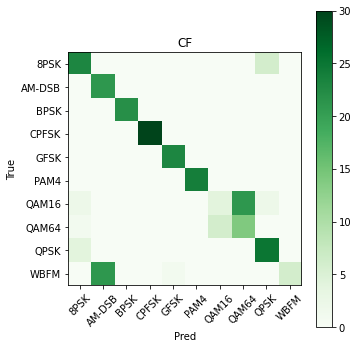
\includegraphics[width=320pt]{imgs/snrs/snr11.png}
\end{center}
\subsubsection{At SNR 12}
\begin{center}
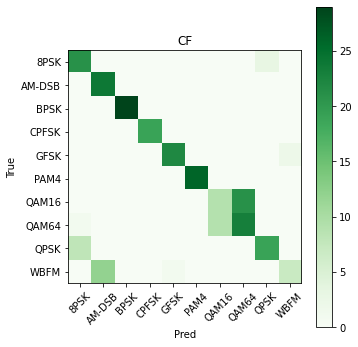
\includegraphics[width=320pt]{imgs/snrs/snr12.png}
\end{center}
\subsubsection{At SNR 14}
\begin{center}
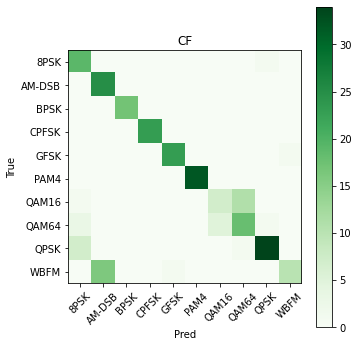
\includegraphics[width=320pt]{imgs/snrs/snr13.png}
\end{center}
\subsubsection{At SNR 16}
\begin{center}
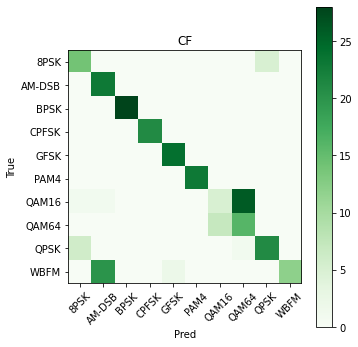
\includegraphics[width=320pt]{imgs/snrs/snr14.png}
\end{center}
\subsubsection{At SNR 18}
\begin{center}
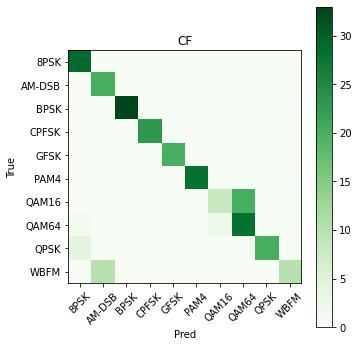
\includegraphics[width=320pt]{imgs/snrs/snr15.png}
\end{center}

\subsubsection{Plots for Some NN Training}
OurCNN-raw-10-epochs
\begin{center}
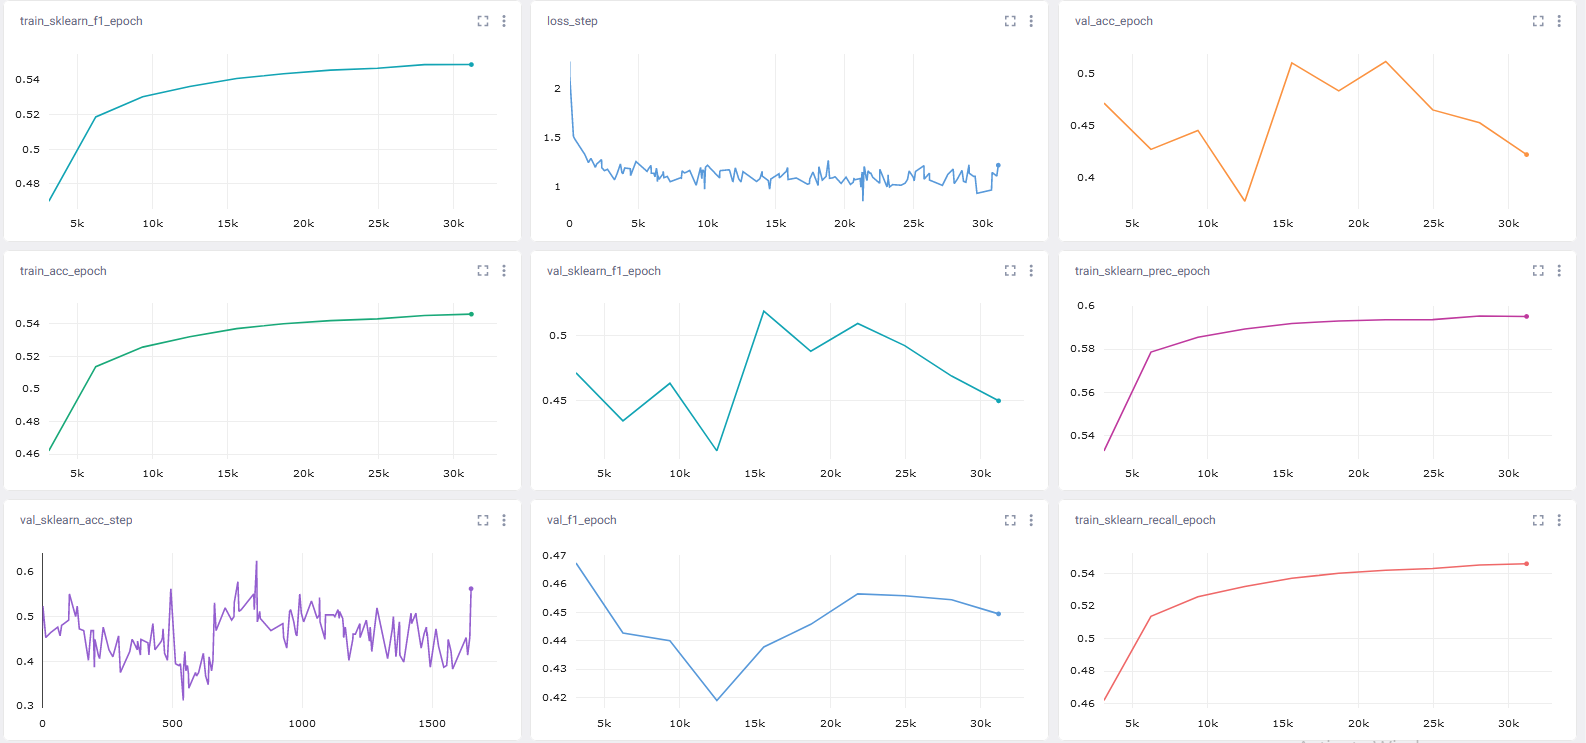
\includegraphics[width=320pt]{imgs/comet1.png}
\end{center}
\newpage
OurCNN-raw-10epochs-b256-lr0.0005-weighted
\begin{center}
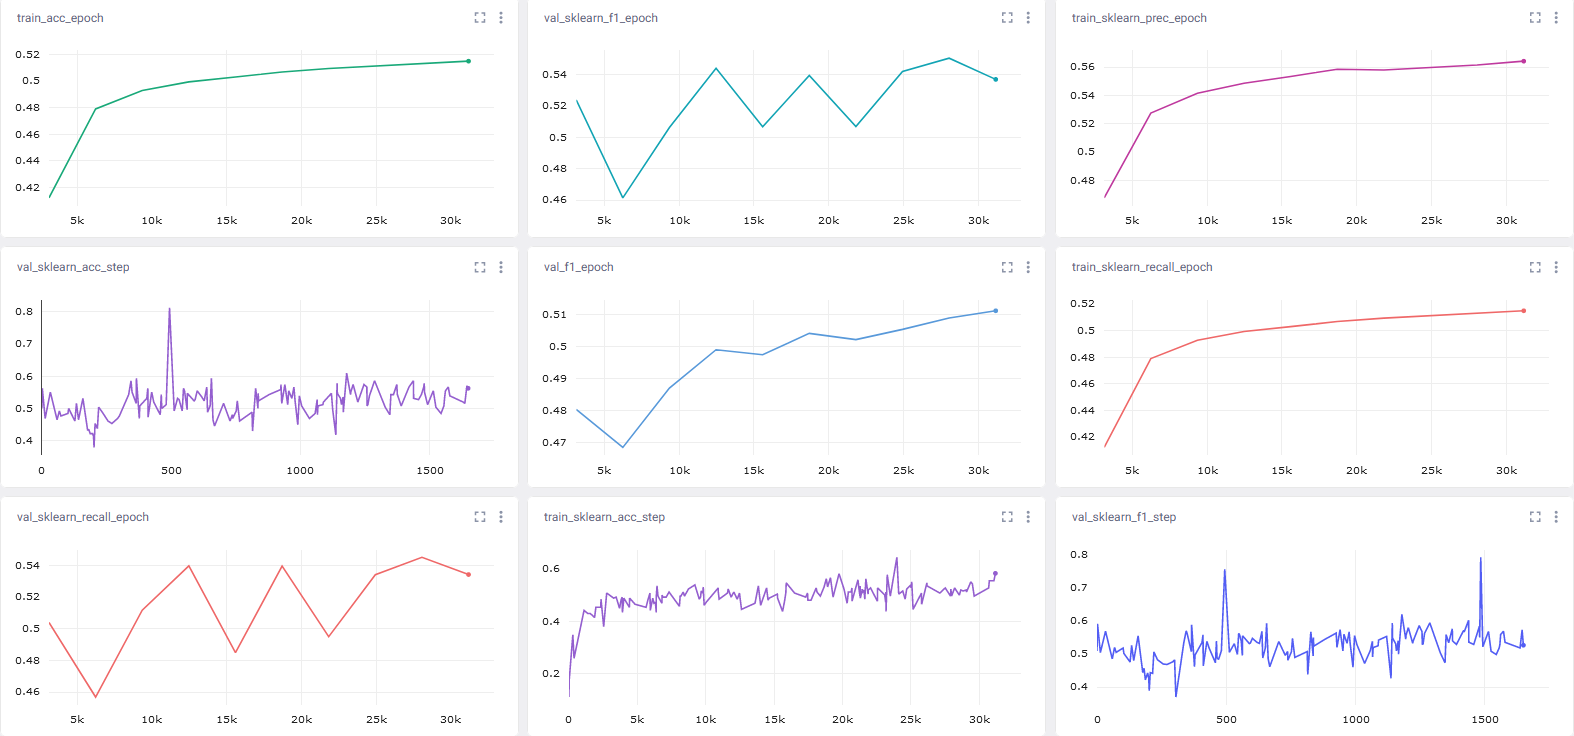
\includegraphics[width=320pt]{imgs/comet2.png}
\end{center}
OurLSTM-raw-10epochs-b256-lr0.001-weighted
\begin{center}
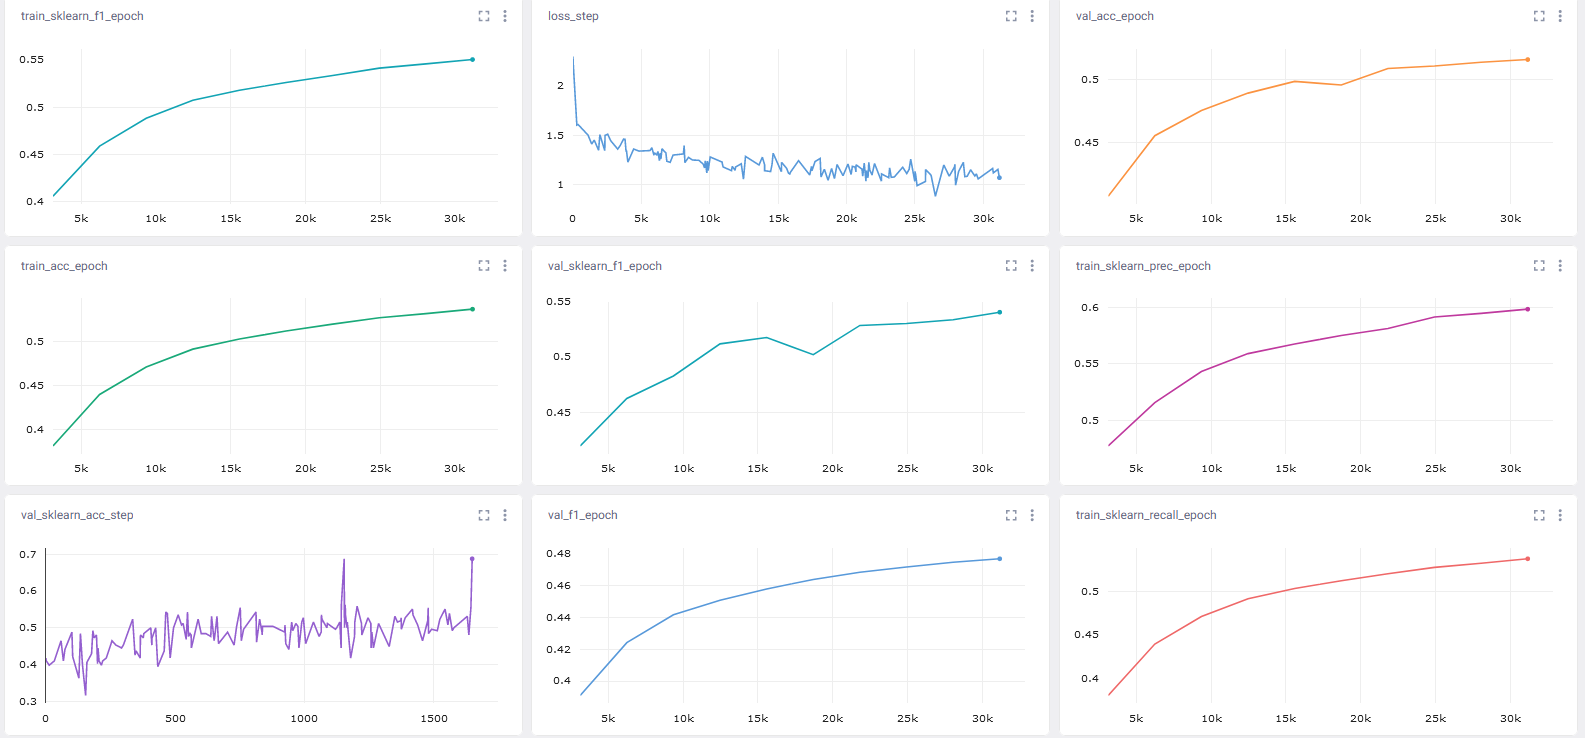
\includegraphics[width=320pt]{imgs/comet3.png}
\end{center}


        
        \newpage
    \section{Conclusion}
    \begin{itemize}
  \item Raw is better than derivative.
  \item CNN and LSTM are usually better than Vanillar RNN.
\end{itemize}

    


    \bibliographystyle{ieeetrans}
    \bibliography{Assignment_Ref}

\end{document}